\documentclass[zihao=false,fontset=windows]{ctexart}
% ctexart 不接受任意 pt 选项。正文改 {10pt}，方括号里是行距。
\usepackage{scrextend}
\changefontsizes[12pt]{10pt}

\usepackage[a4paper,left=2.35cm,right=2.35cm,top=1.7cm,bottom=1.9cm]{geometry}
\usepackage{xcolor}
\usepackage{graphicx}
\usepackage{amsmath,amssymb}
\usepackage{enumitem}
\usepackage{tabularx}
\usepackage{colortbl}
\usepackage{listings}
\usepackage{hyperref}
\usepackage[most]{tcolorbox}

\definecolor{feishuText}{RGB}{31,35,41}
\definecolor{feishuBlue}{RGB}{36,91,219}
\definecolor{feishuRed}{RGB}{216,57,49}
\definecolor{feishuGray}{RGB}{100,106,115}
\definecolor{feishuGray2}{RGB}{143,149,158}
\definecolor{feishuPinkBg}{RGB}{251,191,188}
\definecolor{quoteBar}{RGB}{51,112,255}
\definecolor{codebg}{RGB}{245,246,247}
\definecolor{codeborder}{RGB}{222,224,227}
\definecolor{inlinebg}{RGB}{242,243,245}
\definecolor{callRed}{RGB}{253,226,226}
\definecolor{callOrange}{RGB}{255,245,235}
\definecolor{callYellow}{RGB}{254,255,240}
\definecolor{callGreen}{RGB}{240,251,239}
\definecolor{callBlue}{RGB}{240,244,255}
\definecolor{callRedSoft}{RGB}{254,241,241}
\definecolor{callSun}{RGB}{255,255,204}
\definecolor{tableHead}{RGB}{242,243,245}
\definecolor{tableRule}{RGB}{222,224,227}
\definecolor{codeText}{RGB}{31,35,41}
\definecolor{codeKeyword}{RGB}{0,0,255}
\definecolor{codeComment}{RGB}{0,128,0}
\definecolor{codeString}{RGB}{163,21,21}

\setmainfont{Times New Roman}
\setCJKmainfont{Microsoft YaHei}[AutoFakeBold=2.2]
\setCJKsansfont{Microsoft YaHei}[AutoFakeBold=2.2]
\setCJKmonofont{Microsoft YaHei}[AutoFakeBold=2.2]
\setmonofont{Consolas}
\newfontfamily\emojifont{Segoe UI Emoji}

\hypersetup{
  colorlinks=true,
  urlcolor=feishuBlue,
  linkcolor=feishuBlue,
  unicode=true,
  pdftitle={AIMv2}
}

\setlength{\parindent}{0pt}
\setlength{\parskip}{0.42em}
\setlength{\fboxsep}{1.5pt}
\setlength{\emergencystretch}{3em}
\linespread{1.28}
\color{feishuText}
\arrayrulecolor{tableRule}
\urlstyle{same}

\setlist[enumerate]{label=\textcolor{feishuBlue}{\arabic*.}, leftmargin=1.7em, itemsep=0.22em, topsep=0.28em, parsep=0.08em, partopsep=0pt}
\setlist[itemize,1]{label=\textcolor{feishuBlue}{\textbullet}, leftmargin=1.35em, itemsep=0.18em, topsep=0.25em, parsep=0.06em, partopsep=0pt}
\setlist[itemize,2]{label=\textcolor{feishuBlue}{◦}, leftmargin=1.45em, itemsep=0.12em, topsep=0.15em}
\setlist[itemize,3]{label=\textcolor{feishuBlue}{\rule[0.18em]{0.38em}{0.38em}}, leftmargin=1.55em, itemsep=0.1em, topsep=0.12em}

\newcommand{\feiEmoji}[1]{{\emojifont #1}}
\newcommand{\incode}[1]{\colorbox{inlinebg}{\ttfamily\small #1}}
\newcommand{\bigmath}[1]{%
  \begin{center}\large$\displaystyle #1$\end{center}%
}

\lstset{
  language=Python,
  basicstyle=\ttfamily\footnotesize\color{codeText},
  keywordstyle=\color{codeKeyword},
  commentstyle=\color{codeComment},
  stringstyle=\color{codeString},
  showstringspaces=false,
  breaklines=true,
  columns=fullflexible,
  keepspaces=true,
  tabsize=4,
  upquote=true,
  aboveskip=2pt,
  belowskip=0pt,
  xleftmargin=0pt,
  frame=none
}

\tcbset{
  feishubase/.style 2 args={
    enhanced,
    boxrule=0pt,
    arc=8pt,
    left=10pt,
    right=10pt,
    top=7pt,
    bottom=7pt,
    before skip=6pt,
    after skip=6pt,
    colback=#1,
    colframe=#1,
    before upper={\feiEmoji{#2}\hspace{0.45em}\ignorespaces}
  }
}
\newtcolorbox{feishubox}[2]{feishubase={#1}{#2}, breakable}
\newtcolorbox{feishuboxnb}[2]{feishubase={#1}{#2}}

\newtcolorbox{feishuquote}{
  enhanced,
  breakable,
  boxrule=0pt,
  leftrule=3pt,
  arc=0pt,
  colframe=quoteBar,
  colback=white,
  left=8pt,
  right=2pt,
  top=2pt,
  bottom=2pt,
  before skip=4pt,
  after skip=4pt,
  before upper=\color{feishuGray}
}

\newtcolorbox{feishucode}{
  enhanced,
  breakable,
  colback=codebg,
  colframe=codeborder,
  boxrule=0.6pt,
  arc=6pt,
  left=6pt,
  right=6pt,
  top=5pt,
  bottom=4pt,
  before skip=6pt,
  after skip=6pt
}


\usepackage{needspace}
% 来源：https://scnajei2ds6y.feishu.cn/wiki/XJAmwsJC2iMonCkzvkoc5wgMnIg
% 公式依据网页渲染人工转写；原文Casual标题及Ltext+alpha Ltext保留。

\begin{document}

{\zihao{1}\bfseries AIMv2\par}

\begin{feishubox}{callGreen}{☘}论文：\href{https://arxiv.org/pdf/2411.14402}{《Multimodal Autoregressive Pre-training of Large Vision Encoders》}\par 代码仓库：\href{https://github.com/apple/ml-aim}{apple/ml-aim}\par 模型仓库：\href{https://huggingface.co/collections/apple/aimv2}{apple/aimv2}\end{feishubox}

\textcolor{feishuRed}{\textbf{2025年初主流 MLLM 使用的 Vision Encoder 都是使用判别式任务（对比学习的方法）进行训练的}}，如\href{https://scnajei2ds6y.feishu.cn/wiki/FKvTwjSHxiVHBokxd5ncXxuanch}{CLIP(2021, OpenAI)}、\href{https://scnajei2ds6y.feishu.cn/wiki/IAqAwbiLVi0gEOkC87Qc0hAVnPe}{SigLIP}、\href{https://scnajei2ds6y.feishu.cn/wiki/H3biwpNrQiAgk2kd9bscXeS2nkb}{SigLIP2}，\href{https://scnajei2ds6y.feishu.cn/wiki/SXzcw2VtHig3bPkRfIickYa8nVh}{InternViT}会在判别式任务后加上生成式任务。\par

背景：\par

\begin{itemize}
\item 对比学习参数高效，都是进一步训练scaling难度大。
\item 利用生成式任务进行CV预训练效果不好，达到同样效果通常要数倍参数于对比学习。
\end{itemize}

AIMv2 提出了一种\textcolor{feishuRed}{\textbf{基于多模态自回归的新型 Vision Encoder 预训练框架}}，通过统一处理图像与文本进行视觉预训练。\par

\par\needspace{5\baselineskip}\vspace{1em}\noindent{\zihao{-2}\bfseries \textcolor{feishuBlue}{1.} 模型架构}\par\vspace{0.28em}

模型训练的架构如图（左下）所示，为什么说是“训练的架构”，因为\textcolor{feishuRed}{我们预训练的目标模块是 Prefix Vision Encoder}，但是需要引入 Casual Multimodal Decoder（语言模型）来进行预训练。而右边是 Prefix Vision Encoder 的内部构造。\par

\begin{tcbraster}[raster columns=100,raster equal height=rows,raster column skip=0pt,raster before skip=4pt,raster after skip=4pt]
\begin{tcolorbox}[blankest,raster multicolumn=59,right=4.5pt,valign=top]
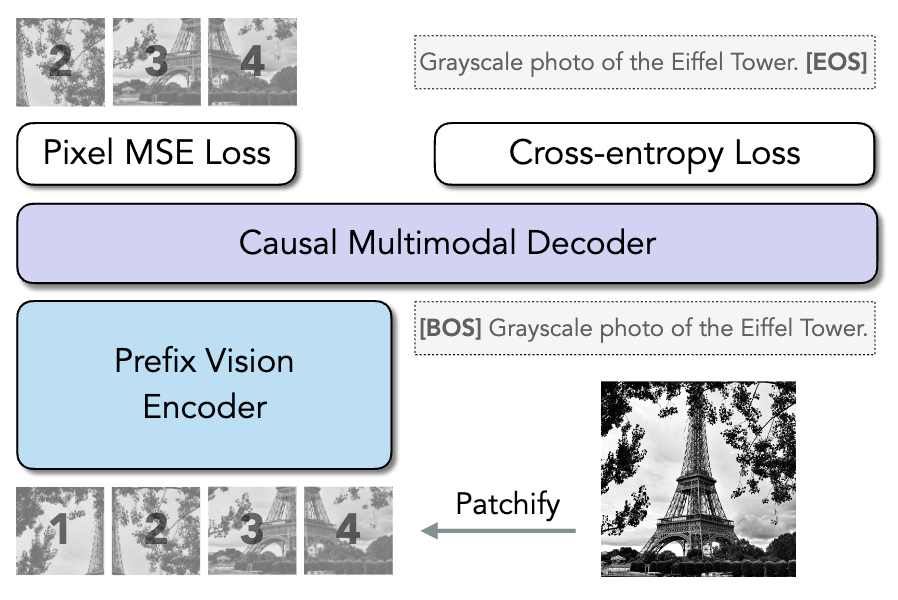
\includegraphics[width=\linewidth]{images/AIMv2/fig-01.png}\par
\begin{center}\color{feishuGray}\small 训练架构\end{center}
\end{tcolorbox}
\begin{tcolorbox}[blankest,raster multicolumn=41,left=4.5pt,valign=top]
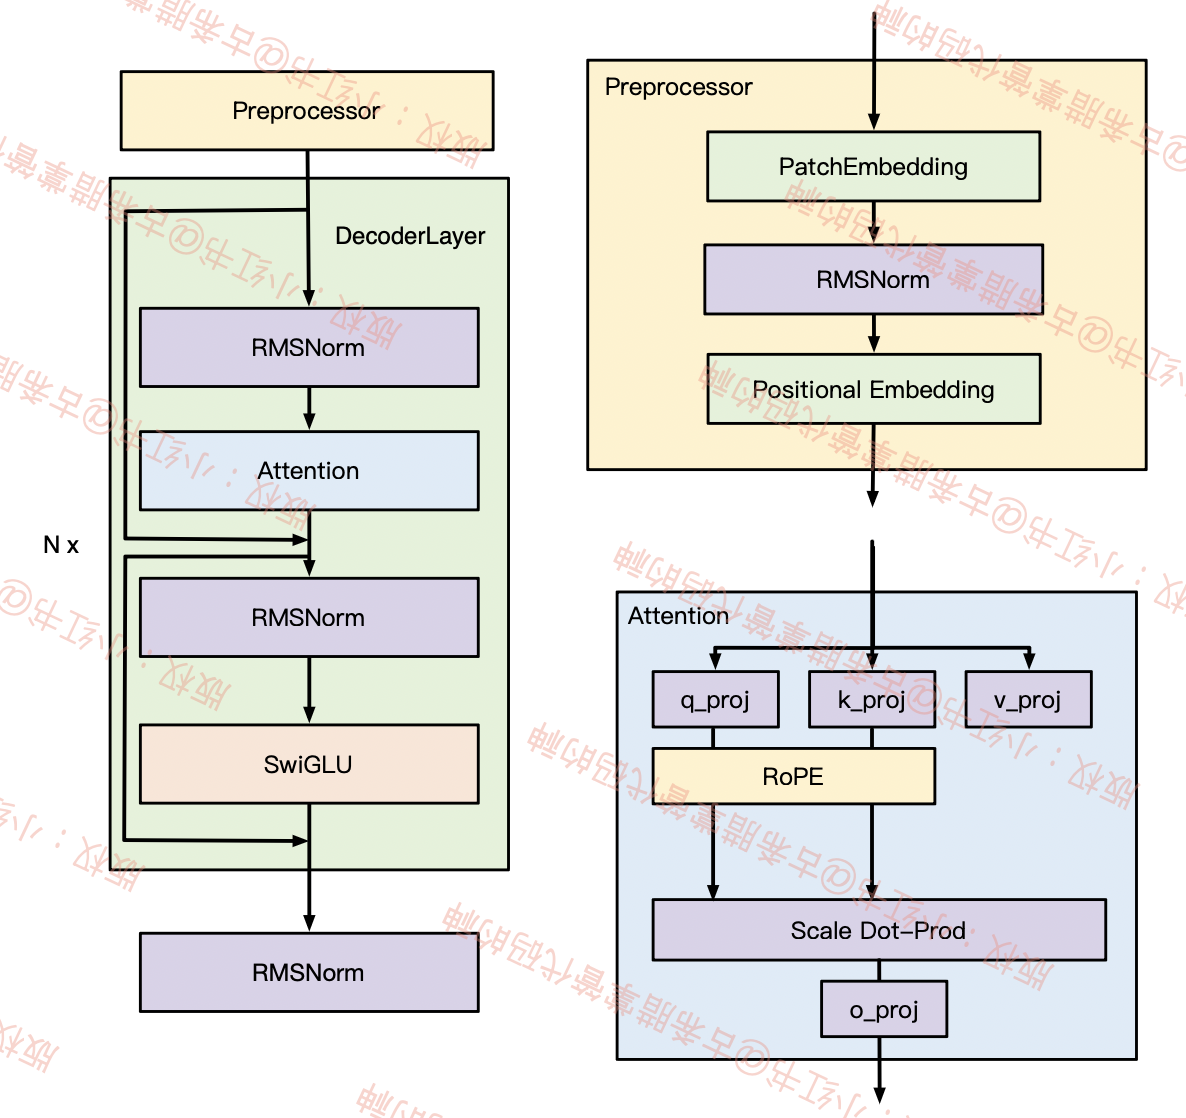
\includegraphics[width=\linewidth]{images/AIMv2/fig-02.png}\par
\begin{center}\color{feishuGray}\small Vision Encoder\end{center}
\end{tcolorbox}
\end{tcbraster}

从左侧训练架构来看，和现在的 MLLM 的架构非常类似，\textcolor{feishuRed}{区别在于在视觉部分全部的feature都会透出到LLM一侧并且计算 MSE Loss，从LLM到输出上观察，语言和视觉都是通过 Next Token Prediction 进行训练了}，我们将依据左图架构分别介绍各个模块（以及Loss）。\par

\par\needspace{5\baselineskip}\vspace{1em}\noindent{\zihao{3}\bfseries \textcolor{feishuBlue}{1.1} Prefix Vision Encoder}\par\vspace{0.28em}

\begin{center}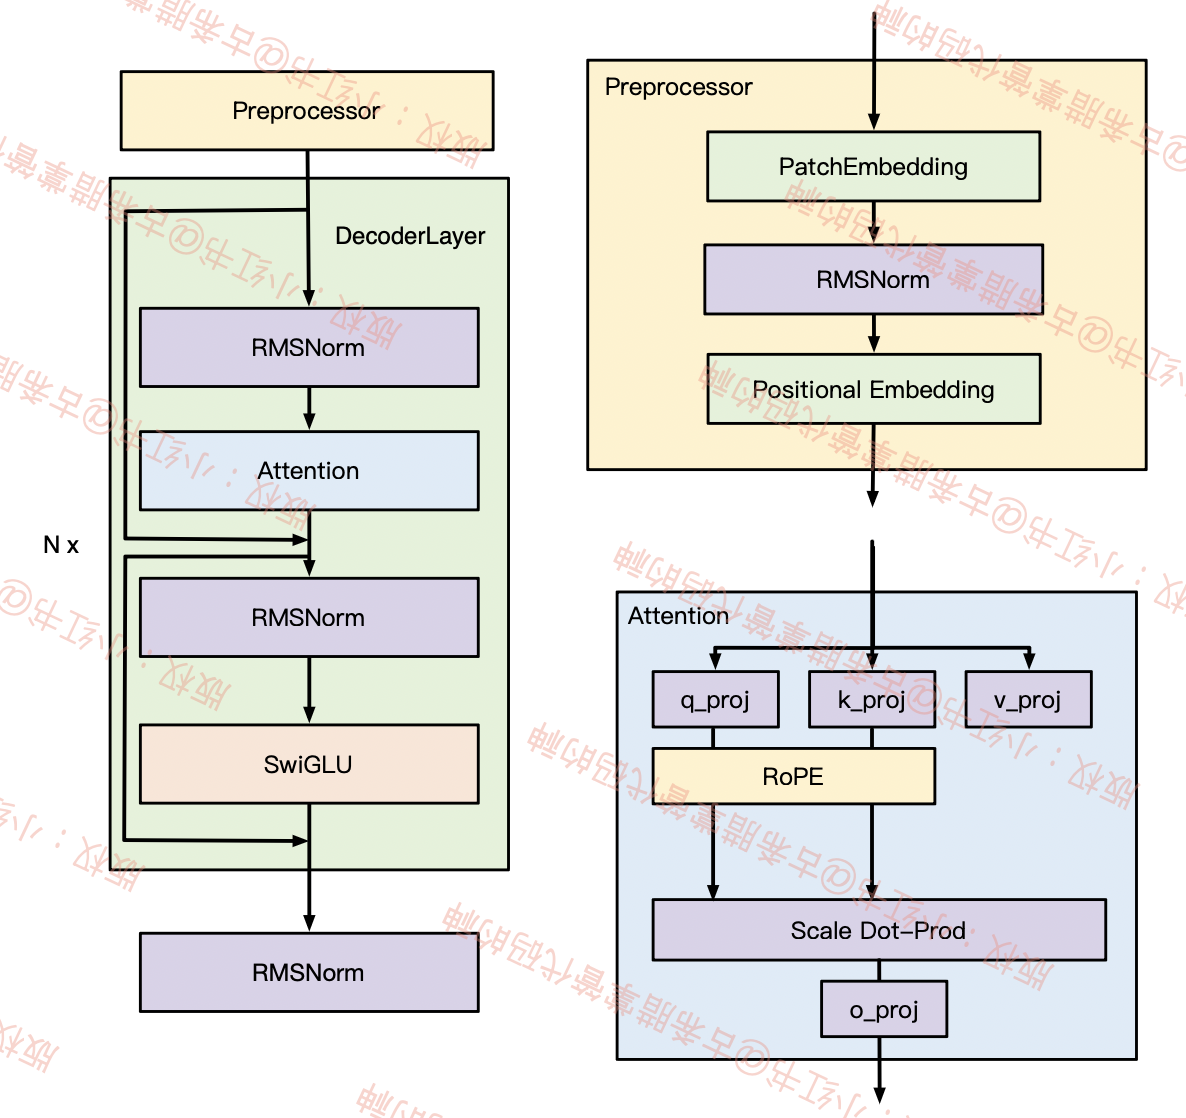
\includegraphics[width=0.68\linewidth]{images/AIMv2/fig-03.png}\end{center}

Vision Encoder 的架构本质是一个 \href{https://scnajei2ds6y.feishu.cn/wiki/QEJ8wXq9GiTBrxkMqbScnd8nnod}{ViT(2020, Google Research)}，但是同 \href{https://scnajei2ds6y.feishu.cn/wiki/S7Q2wviQhiYtQFk4jKvccQwDnWe}{Qwen2.5-VL}一样，\textcolor{feishuRed}{\textbf{AIMv2的 ViT 使用了更接近语言模型的架构}}：RMSNorm + SwiGLU 结构的 FFN\par

具体来说，归一化层 (Norm) 相比 ViT 的 LayerNorm 替换为了 \textbf{RMSNorm}（Root Mean Square Normalization）：\par

\begin{feishucode}
\begin{lstlisting}[numbers=left,numberstyle=\tiny\color{feishuGray},numbersep=6pt,xleftmargin=12pt]
class RMSNorm(nn.Module):
    def __init__(self, dim: int, eps: float = 1e-6):
        super().__init__()
        self.weight = nn.Parameter(torch.ones(dim))
        self.eps = eps

    def forward(self, x: torch.Tensor) -> torch.Tensor:
        output = self._norm(x.float()).type_as(x)
        return output * self.weight

    def extra_repr(self) -> str:
        return f"{tuple(self.weight.shape)}, eps={self.eps}"

    def _norm(self, x: torch.Tensor) -> torch.Tensor:
        return x * torch.rsqrt(x.pow(2).mean(-1, keepdim=True) + self.eps)
\end{lstlisting}
\end{feishucode}

以及FFN使用了SwiGLU的结构，\textcolor{feishuRed}{\textbf{但是相比 }}\textcolor{feishuRed}{\textbf{\href{https://scnajei2ds6y.feishu.cn/wiki/S7Q2wviQhiYtQFk4jKvccQwDnWe}{Qwen2.5-VL}}}\textcolor{feishuRed}{\textbf{没有启用bias：}}\par

\begin{feishucode}
\begin{lstlisting}[numbers=left,numberstyle=\tiny\color{feishuGray},numbersep=6pt,xleftmargin=12pt]
class AIMv2SwiGLUFFN(nn.Module):
    def __init__(self, config: AIMv2Config):
        super().__init__()
        hidden_features = config.intermediate_size
        in_features = config.hidden_size
        bias = config.use_bias

        self.fc1 = nn.Linear(in_features, hidden_features, bias=bias)
        self.fc2 = nn.Linear(hidden_features, in_features, bias=bias)
        self.fc3 = nn.Linear(in_features, hidden_features, bias=bias)

    def forward(self, x: torch.Tensor) -> torch.Tensor:
        x = F.silu(self.fc1(x)) * self.fc3(x)
        x = self.fc2(x)
        return x
\end{lstlisting}
\end{feishucode}

Attention 使用的是标准的 \incode{F.scaled\_dot\_product\_attention}，位置编码使用的是\textcolor{feishuRed}{\textbf{固定位置编码}}（参考\href{https://scnajei2ds6y.feishu.cn/wiki/O2arwxGNXi6KrckUG1dcGcbrnWd}{ViT的位置编码}），不过AIMv2也提供了兼容\href{https://scnajei2ds6y.feishu.cn/wiki/N6PmwVkCcisDJGkC7Ypc1SfInwh}{NaViT}动态位置编码的版本，可以参考\href{https://huggingface.co/apple/aimv2-large-patch14-native/blob/main/modeling_aimv2.py}{代码}。\par

\par\needspace{5\baselineskip}\vspace{1em}\noindent{\zihao{3}\bfseries \textcolor{feishuBlue}{1.2} Casual Multimodal Decoder}\par\vspace{0.28em}

Causal Multimodal Decoder采用了一个基于Transformer架构的自回归多模态解码器，\textcolor{feishuRed}{\textbf{但是并没有说使用的具体模型来源}}。该解码器将图像特征（来自Vision Transformer编码器）与文本token的嵌入向量进行线性投影后拼接，形成统一的输入序列。图像和文本token通过共享的Transformer层进行处理，使用因果注意力机制（causal attention mask）确保自回归生成特性。\par

\textcolor{feishuRed}{\textbf{解码器末端包含两个独立线性投影头：}}\par

\begin{itemize}
\item 图像头：预测未归一化的图像像素块（使用MSE损失）
\item 文本头：预测文本token的概率分布（使用交叉熵损失）
\end{itemize}

这种设计允许同时进行图像和文本的生成和Loss计算。\par

\par\needspace{5\baselineskip}\vspace{1em}\noindent{\zihao{3}\bfseries \textcolor{feishuBlue}{1.3} Loss}\par\vspace{0.28em}

Vision Encoder 连续 Patch 序列（\mbox{$x_i\in\mathbb R^I$}）与文本子词序列（\mbox{$x_t\in\mathbb R^T$}）拼接为统一输入序列，通过多模态解码器自回归\textcolor{feishuRed}{\textbf{分别}}生成图像块与文本标记。\par

\begin{tcbraster}[raster columns=2,raster equal height=rows,raster column skip=9pt]
\begin{tcolorbox}[blankest,valign=top]
损失函数包含两个部分：\par\begin{itemize}
\item 图像像素回归损失\mbox{$\displaystyle\mathcal L_{img}=\sum_{i=1}^{I}\|\hat x_i-x_i\|_2^2$}
\item 文本交叉熵损失\mbox{$\displaystyle\mathcal L_{text}=-\sum_{t=I+1}^{I+T}\log P(x_t|x_{<t})$}
\end{itemize}通过比例因子$\alpha$进行加权获得最终的 Loss：\par\bigmath{\mathcal L=\mathcal L_{text}+\alpha\mathcal L_{text}\text{。}}\par\begin{feishuquote}\mbox{$\alpha=0.4$}达到最优。\end{feishuquote}
\end{tcolorbox}
\begin{tcolorbox}[blankest,valign=top]
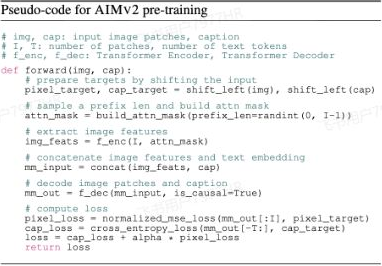
\includegraphics[width=\linewidth]{images/AIMv2/fig-04.png}
\end{tcolorbox}
\end{tcbraster}

\par\needspace{5\baselineskip}\vspace{1em}\noindent{\zihao{-2}\bfseries \textcolor{feishuBlue}{2.} 预训练\&后训练}\par\vspace{0.28em}

\begin{itemize}
\item \textbf{预训练}：使用 12B 图像-文本对（224x224），包含公开数据集（DFN-2B、COYO）与私有高质量数据（HQITP），结合合成标注增强多样性。  
\item \textbf{后训练：}使用 2B 量级 336px和448px分辨率图像（与预训练数据同源，不含合成标注），\href{https://scnajei2ds6y.feishu.cn/wiki/N6PmwVkCcisDJGkC7Ypc1SfInwh}{NaViT}架构模型进行动态分辨率Packing训练。
\item \textbf{可扩展性}：模型参数范围300M至3B，实验表明数据与模型容量同步扩展时性能持续提升，尤其在计算资源充足时大模型优势显著（如3B模型在IN-1k达到89.5\%准确率）。  
\end{itemize}

\begin{center}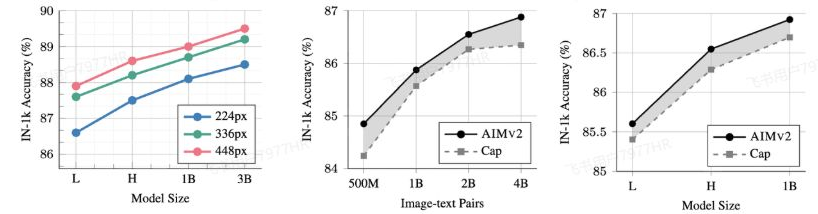
\includegraphics[width=0.98\linewidth]{images/AIMv2/fig-05.png}\end{center}

\par\needspace{5\baselineskip}\vspace{1em}\noindent{\zihao{-2}\bfseries \textcolor{feishuBlue}{3.} 实验}\par\vspace{0.28em}

\begin{itemize}\item \textbf{视觉任务}：  \begin{itemize}
\item \textbf{图像分类}：冻结主干的AIM V2-3B在IN-1k达到89.5\%准确率，超越MAE、DINOv2等自监督方法。  
\item \textbf{目标检测与定位}：在COCO、LVIS等基准中，OVD与REC任务上显著优于DINOv2与CLIP模型。  
\end{itemize}\end{itemize}

\begin{center}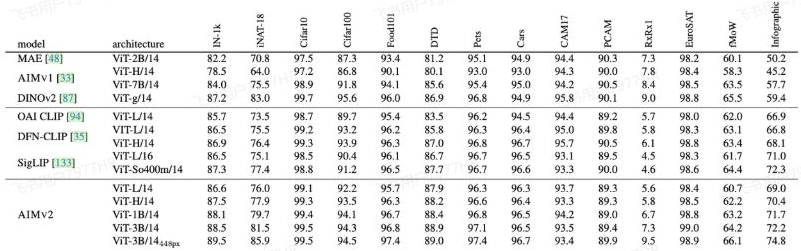
\includegraphics[width=0.98\linewidth]{images/AIMv2/fig-06.png}\end{center}

\begin{itemize}\item \textbf{多模态理解}：  \begin{itemize}
\item \textbf{指令微调}：结合LLM（如Llama 3）进行单阶段微调，在VQAv2、TextVQA等问答任务中优于SigLIP与CLIP，且支持高分辨率分块推理（最高1008px）。 
\item \textbf{上下文学习}：在4/8样本少样本设置下，多模态ICL性能超越MM1系列模型，验证其与大规模多模态管道的兼容性。  
\end{itemize}\end{itemize}

\begin{center}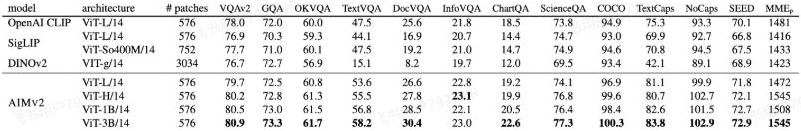
\includegraphics[width=0.98\linewidth]{images/AIMv2/fig-07.png}\end{center}

\end{document}
